\documentclass[conference]{IEEEtran}
\IEEEoverridecommandlockouts
\usepackage{cite}
\usepackage{amsmath,amssymb}
\usepackage{graphicx}
\usepackage{booktabs}
\usepackage{multirow}
\usepackage{xcolor}
\usepackage{tikz}
\usetikzlibrary{arrows.meta,positioning,fit,calc,shapes.geometric}
\usepackage[hidelinks]{hyperref}

% values that can only be measured on the board
\newcommand{\tbd}[1]{\textcolor{red}{#1}}

\setlength{\textfloatsep}{8pt plus 2pt minus 2pt}
\setlength{\floatsep}{6pt plus 2pt minus 2pt}
\setlength{\dblfloatsep}{6pt plus 2pt minus 2pt}
\setlength{\dbltextfloatsep}{8pt plus 2pt minus 2pt}
\renewcommand{\arraystretch}{0.93}
\linespread{0.985}
\begin{document}

\title{FPGA-Based Real-Time Moving Object Detection Using Gaussian Mixture Model
Background Subtraction and Single-Pass Connected Component Labeling on Zynq SoC}

\maketitle

\begin{abstract}
We present a moving object detector on a Zynq-7000 system-on-chip. It builds on
the hardware-oriented OpenCV Gaussian mixture model (GMM) of Genovese and
Napoli. Their background circuit is re-implemented as a pipeline that takes one
pixel per clock. We extend it with a configurable $3\times3$ morphological
filter, a single-pass connected component labeling (CCL) unit that returns the
bounding box and area of every object without storing a labeled image, and an
AXI DMA and AXI4-Lite interface. The per-pixel model stays in DDR memory, so the
ARM cores only read the object list. A software warm-up schedule for the
power-of-two learning rate speeds up the first learning of the model. The RTL
matches a fixed-point reference model bit for bit, also under random stream
stalls. In a word-length study, the 99-bit representation of the
original paper meets the paper's pixel-mismatch target, yet it produces many
false objects after blob analysis. A 126-bit representation fits one 128-bit DMA
word, differs from the floating-point algorithm in only 0.25\% of the pixels and
reaches an F1 score of 0.984 on a sequence with exact ground truth. After place
and route in Vivado, the core uses 3.8k LUTs, which is 7.2\% of the Zynq-7020. It
meets timing at 100\,MHz, its datapath needs 3.10\,ms per $640\times480$ frame
and its estimated dynamic power is 43\,mW. On a PYNQ-Z2 board, the hardware path
processes VGA video at 115\,frames/s, 15.5 times faster than the ARM software,
and matches the model bit for bit.
\end{abstract}

\begin{IEEEkeywords}
FPGA, Zynq, background subtraction, Gaussian mixture model, OpenCV,
connected component labeling, moving object detection, PYNQ
\end{IEEEkeywords}

%=============================================================================
\section{Introduction}
%=============================================================================
Most video surveillance and traffic monitoring systems start from a static
camera, and their first task is to find what moves. Background subtraction
separates the moving foreground from the scene. A blob analysis then turns the
foreground mask into individual objects.

Gaussian mixture models (GMMs)~\cite{stauffer1999,kaew2001} describe each pixel
with several Gaussians. This lets them cope with slow lighting changes and with
backgrounds that repeat, such as waving leaves or flickering screens. OpenCV
ships a GMM variant that learns its first model quickly. It keeps a match
counter for every Gaussian, and the learning rate depends on the weight of each
Gaussian~\cite{genovese2014}.

The model is costly. For every pixel of every frame, the system reads $K$
Gaussians, matches, orders and updates them, and writes them back. Classic
connected component labeling is costly too, since it needs two raster passes and
a label frame buffer~\cite{rosenfeld1966}.

Genovese and Napoli~\cite{genovese2014} reformulated the OpenCV GMM so that its
nonlinear operations reduce to a small look-up and some shifters. They chose the
word lengths of the Gaussian parameters by counting the pixels classified
differently from a double-precision reference, with a target below 0.05. Their
FPGA circuit handles one pixel per clock.

We start from their formulation and build a complete detector around it on a
Zynq-7000 SoC~\cite{ug585}. Our contributions are:
\begin{itemize}\setlength{\itemsep}{0pt}\setlength{\parsep}{0pt}\setlength{\topsep}{1pt}
\item a pipelined RTL version of the GMM in~\cite{genovese2014} with
      parameterized word lengths, a multiplier-and-comparator learning-rate
      look-up and a software warm-up schedule;
\item a streaming morphology chain that tolerates stalls and performs closing,
      opening or both;
\item a two-stage single-pass CCL unit with a fully resolved merger table. It
      outputs bounding boxes and areas at the end of each frame;
\item integration with AXI DMA and AXI4-Lite on PYNQ-Z1/Z2 and other Zynq-7020
      boards, with PYNQ and bare-metal software;
\item a bit-exact verification flow and a word-length study. The study checks
      the pixel-level agreement with the floating-point algorithm and the
      object-level detection quality.
\end{itemize}

%=============================================================================
\section{Related Work}
%=============================================================================
Stauffer and Grimson rank the Gaussians of each pixel by their fitness
$w/\sigma$. The highest-ranked ones form the background~\cite{stauffer1999}.
KaewTraKulPong and Bowden improved the initial learning phase~\cite{kaew2001}.
Zivkovic made the number of components per pixel adaptive~\cite{zivkovic2004},
which is OpenCV's MOG2.

Several hardware designs exist. Jiang \emph{et al.} reduced the memory bandwidth
of the parameter stream~\cite{jiang2009}, and Kristensen \emph{et al.} built a
complete surveillance system with GMM segmentation~\cite{kristensen2008}.
Genovese and Napoli first implemented the OpenCV GMM with ROM-based nonlinear
functions and added morphological denoising~\cite{genovese2012}. Later they
introduced the inverse-fitness formulation that we use here. It runs at 189\,MHz
on a Virtex-6 and delivers 91 HD frames per second~\cite{genovese2014}. Kryjak
\emph{et al.} put GMM-style segmentation into an FPGA surveillance
system~\cite{kryjak2011}. For labeling, Bailey and Johnston showed a one-pass
method that gathers region features while labels are assigned~\cite{bailey2007}. FPGA versions~\cite{johnston2008} followed, and later
work reduced the overhead at the end of each row~\cite{ma2008,bailey2019}.

%=============================================================================
\section{Algorithm}
%=============================================================================
\subsection{OpenCV GMM in the Formulation of~\cite{genovese2014}}
Each pixel is modeled by $K=3$ Gaussians. Gaussian $k$ has a weight $w_k$, a
mean $\mu_k$, a variance $\sigma_k^2$ and a match counter $c_k$
(\emph{matchsum}). It matches the luminance $x$ if
\begin{equation}
(x-\mu_k)^2 < \lambda^2\sigma_k^2,\qquad \lambda=2.5 .
\label{eq:match}
\end{equation}
More than one Gaussian can match. The matched Gaussian $m$ is the one with the
highest fitness $F_k=w_k/\sigma_k$ among them. It is updated as
\begin{align}
\mu_m &\leftarrow \mu_m+\alpha_m(x-\mu_m),\nonumber\\
\sigma_m^2 &\leftarrow \sigma_m^2+\alpha_m\big((x-\mu_m)^2-\sigma_m^2\big),\nonumber\\
w_m &\leftarrow w_m-\alpha_w w_m+\alpha_w, \qquad c_m\leftarrow c_m+1,
\label{eq:upd}
\end{align}
while the other weights decay as $w_k\leftarrow w_k-\alpha_w w_k$. In OpenCV the
learning rate of a Gaussian depends on its weight: $\alpha_k=\alpha_w/w_k$. A
new Gaussian therefore learns fast.

If no Gaussian matches, the one with the lowest fitness is replaced. The new
values are $(w,\mu,\sigma^2,c)=(1/c_{\text{tot}},\,x,\,\sigma_{\text{init}}^2,\,1)$,
where $c_{\text{tot}}$ is the sum of the matchsums of the other two Gaussians.
To find the background, order the Gaussians by fitness and add their weights in
that order. The first $B$ Gaussians whose weights together exceed $T=0.7$ form
the background. A pixel is background when it matches one of them.

Genovese and Napoli remove the nonlinear operations in two steps. They quantize
both learning rates to powers of two, $\alpha_w=2^{-a}$ and
$\alpha_k=2^{-s_k}$. They also order the Gaussians by the inverse fitness
\begin{equation}
IF_k = \Big(\frac{\sigma_k}{w_k}\Big)^{2}=\sigma_k^2\,\Big(\frac{\alpha_k}{\alpha_w}\Big)^{2}
=\sigma_k^2\cdot 2^{\,2(a-s_k)} ,
\label{eq:if}
\end{equation}
so a single shifter replaces two multipliers and a square root~\cite{genovese2014}.
In their circuit $s_k$ comes from a ROM indexed by $w_k$.

\subsection{Implementation Choices}
\emph{Learning-rate look-up.} Let the weight code $c_w$ have $W_B$ bits. Then
$s_k=\max\!\big(0,\;a-W_B+\operatorname{round}(\log_2 c_w)\big)$. We compute the
rounded logarithm exactly. It equals the number of $r\in[0,W_B)$ with
$c_w\ge 2^{\,r+1/2}$. That takes $W_B$ comparators against constants and no
ROM, so the circuit does not depend on the word length.

\emph{Ordering.} Three comparators rank the three $IF_k$ values. Ties go to the
lower index, and an empty Gaussian ($w_k=0$) gets the largest value. The
background test then reads $\sum_{j:\,\text{rank}_j<\text{rank}_m} w_j \le T$.
\emph{Replacement weight.} The value $1/c_{\text{tot}}$ comes from a small
constant table, since $c_{\text{tot}}\le 30$. \emph{Rounding.} Every shift rounds
half up. This halves the dead zone, the range where an update smaller than one
LSB is lost.

\emph{Warm-up schedule.} The bootstrap model has one Gaussian per pixel, with
$w=1$ and $\sigma^2=\sigma_{\text{init}}^2=900$ (OpenCV uses
$\sigma_{\text{init}}=30$). With a constant $\alpha_w=2^{-7}$ this variance
needs hundreds of frames to shrink. So before frame $t$ the software writes
$a_t=\min(a,\lceil\log_2(t+1)\rceil)$ to the learning-rate register. During the
first $2^a$ frames this gives $\alpha_w\approx 1/t$, in the spirit of the initial
phase of~\cite{kaew2001}. The hardware itself does not change.

\begin{table}[!t]
\caption{Word lengths of the Gaussian parameters}
\label{tab:fxp}
\centering
\begin{tabular}{@{}lccc@{}}
\toprule
Signal & Format & Table I of \cite{genovese2014} & This work (default)\\
\midrule
weight $w_k$            & U$-1,W_B$  & 8  & 12\\
mean $\mu_k$            & U$7,F_M$   & 10 & 12\\
variance $\sigma_k^2$   & U$13,\cdot$ & 11 & 14\\
matchsum $c_k$          & U$3,0$     & 4  & 4\\
\midrule
model bits / pixel      &            & 99 & 126\\
\bottomrule
\end{tabular}
\end{table}

\emph{Word lengths.} All four word lengths are synthesis parameters
(Table~\ref{tab:fxp}). The model of one pixel always fits one 128-bit DMA word.
Our default spends the extra bits on the weight, the mean and the variance, and
the configuration of Table~I of~\cite{genovese2014} stays available.

\subsection{Morphology and Single-Pass CCL}
\begin{figure*}[!t]
\centering
\resizebox{0.9\textwidth}{!}{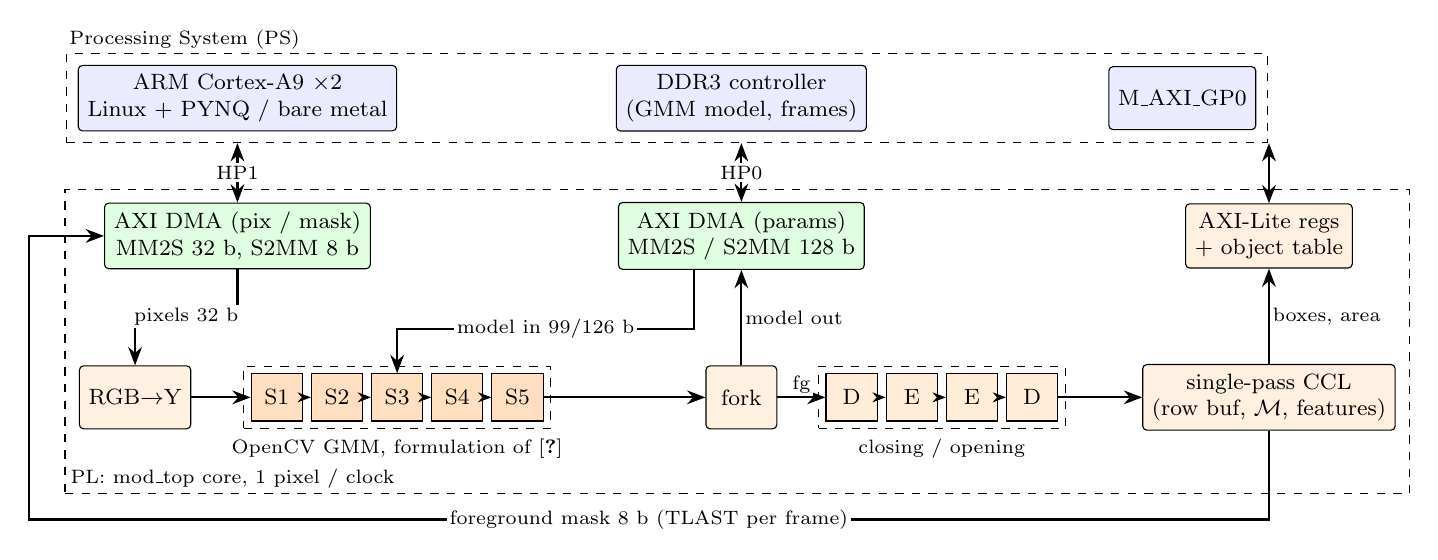
\begin{tikzpicture}[font=\footnotesize, >=Stealth, x=1cm, y=1cm,
  blk/.style={draw, rounded corners=1.5pt, align=center, minimum height=8mm, fill=white},
  ps/.style={blk, fill=blue!8}, pl/.style={blk, fill=orange!12}, dma/.style={blk, fill=green!12},
  st/.style={draw, minimum width=6.5mm, minimum height=6mm, fill=orange!25, inner sep=1pt},
  lab/.style={font=\scriptsize, fill=white, inner sep=1pt}]
% ---------------- PS
\node[ps, minimum width=30mm] (arm) at (2.2,4.1) {ARM Cortex-A9 $\times2$\\Linux + PYNQ / bare metal};
\node[ps, minimum width=24mm] (ddr) at (8.6,4.1) {DDR3 controller\\(GMM model, frames)};
\node[ps, minimum width=16mm] (gp)  at (14.2,4.1) {M\_AXI\_GP0};
\node[draw, dashed, fit=(arm)(ddr)(gp), inner sep=4pt] (psb) {};
\node[anchor=south west, font=\scriptsize, inner sep=1pt] at (psb.north west) {Processing System (PS)};
% ---------------- DMA
\node[dma, minimum width=28mm] (dpix) at (2.2,2.35) {AXI DMA (pix / mask)\\MM2S 32 b, S2MM 8 b};
\node[dma, minimum width=28mm] (dpar) at (8.6,2.35) {AXI DMA (params)\\MM2S / S2MM 128 b};
\draw[<->, thick] (dpix.north) -- node[lab]{HP1} (dpix.north|-psb.south);
\draw[<->, thick] (dpar.north) -- node[lab]{HP0} (dpar.north|-psb.south);
% ---------------- core
\node[pl, minimum width=12mm] (y) at (0.9,0.3) {RGB$\to$Y};
\node[st] (s1) at (2.7,0.3) {S1};
\node[st, right=1mm of s1] (s2) {S2};
\node[st, right=1mm of s2] (s3) {S3};
\node[st, right=1mm of s3] (s3b) {S4};
\node[st, right=1mm of s3b] (s4) {S5};
\node[draw, dashed, fit=(s1)(s4), inner sep=2.5pt, label={[font=\scriptsize]below:{OpenCV GMM, formulation of \cite{genovese2014}}}] (gmm) {};
\node[pl, minimum width=9mm] (fork) at (8.6,0.3) {fork};
\node[st, fill=orange!15] (m1) at (10.0,0.3) {D};
\node[st, fill=orange!15, right=1mm of m1] (m2) {E};
\node[st, fill=orange!15, right=1mm of m2] (m3) {E};
\node[st, fill=orange!15, right=1mm of m3] (m4) {D};
\node[draw, dashed, fit=(m1)(m4), inner sep=2.5pt, label={[font=\scriptsize]below:closing / opening}] (mor) {};
\node[pl, minimum width=20mm] (ccl) at (15.3,0.3) {single-pass CCL\\(row buf, $\mathcal{M}$, features)};
\node[pl, minimum width=20mm] (reg) at (15.3,2.35) {AXI-Lite regs\\+ object table};
% ---------------- data flow
\draw[->, thick] (dpix.south) -- ++(0,-0.6) -| node[lab, pos=0.25]{pixels 32 b} (y.north);
\draw[->, thick] (y) -- (s1);
\draw[->] (s1)--(s2); \draw[->] (s2)--(s3); \draw[->] (s3)--(s3b); \draw[->] (s3b)--(s4);
\draw[->, thick] ($(dpar.south)+(-0.6,0)$) -- ++(0,-0.75) -| node[lab, pos=0.25]{model in 99/126 b} (s3.north);
\draw[->, thick] (s4) -- (fork);
\draw[->, thick] (fork.north) -- node[lab, right]{model out} (fork.north|-dpar.south);
\draw[->, thick] (fork) -- node[lab, above]{fg} (m1);
\draw[->] (m1)--(m2); \draw[->] (m2)--(m3); \draw[->] (m3)--(m4);
\draw[->, thick] (m4) -- (ccl);
\draw[->, thick] (ccl.south) -- (15.3,-1.25) -- node[lab, pos=0.5]{foreground mask 8 b (TLAST per frame)} (-0.45,-1.25) |- (dpix.west);
\draw[->, thick] (ccl.north) -- node[lab, right]{boxes, area} (reg.south);
\draw[<->, thick] (reg.north) -- (reg.north|-psb.south);
\coordinate (plbot) at (0.9,-0.75);
\node[draw, dashed, fit=(y)(gmm)(mor)(ccl)(reg)(plbot), inner sep=5pt] (plb) {};
\node[anchor=south west, font=\scriptsize, inner sep=2pt] at (plb.south west) {PL: mod\_top core, 1 pixel / clock};
\end{tikzpicture}}
\caption{System architecture. The per-pixel background model (128 bits) is
streamed from DDR through the GMM pipeline and back every frame. The
foreground mask returns through the second DMA, and the object list is read
over AXI4-Lite.}
\label{fig:system}
\end{figure*}
Four streaming $3\times3$ stages run in a chain: dilate, erode, erode, dilate.
They are enabled in pairs. This gives four modes: no filtering, opening,
closing, and closing followed by opening. Neighbors outside the frame are
ignored.

The CCL unit receives the filtered mask in raster order. For a foreground pixel
it looks at four labeled 8-neighbors: $A$ (up-left), $B$ (up), $C$ (up-right)
and $D$ (left). $A$, $B$ and $C$ come from a row buffer of provisional labels.
$D$ is the previous result.

A merger table $\mathcal{M}$ maps every label to its root. $A$, $B$ and $D$ are
always connected to each other, so at most two roots meet at a pixel. One is
$X$, the first non-zero of $\{B,A,D\}$. The other is $C$.

A pixel with no labeled neighbor gets a new label. A pixel with one root
inherits it. If two different roots meet, the larger root $g$ merges into the
smaller root $s$. In the same cycle, \emph{all} entries $\mathcal{M}[i]=g$
change to $s$. So $\mathcal{M}$ always points directly to roots, and no
end-of-row resolution is needed. A feature table collects the bounding box and area of every label. Merging
features (min, max, sum) is symmetric, so the features of $X$ and $C$ can be
read before the result label is known. After the last pixel, a scan of at most
$L$ cycles copies the roots with area $\ge A_{\min}$ into a 32-entry object
table.

%=============================================================================
\section{Hardware Architecture}
%=============================================================================

\subsection{System Organization}
Fig.~\ref{fig:system} shows the system. One AXI DMA streams the parameter words
in and out through HP0. A second DMA reads the 32-bit RGBX pixels and writes the
8-bit mask through HP1. The core joins the pixel and model streams, then forks
the GMM output into the returned model and the mask path.

All blocks use AXI4-Stream valid/ready handshakes, so a stall travels backwards
without losing data. Both output streams assert TLAST on the last pixel of a
frame. Software keeps two model buffers and swaps them every frame. The memory
traffic per pixel is $4+16+16+1=37$\,B, which is 341\,MB/s at $640\times480$
and 30\,frames/s.

\subsection{GMM Datapath}
The GMM core has five register stages that share one clock enable.

S1 converts RGB to luminance with $Y=(77R+150G+29B)\gg 8$. The paper also feeds
its circuit with luminance~\cite{genovese2014}. S1 also unpacks the model. S2
computes $x-\mu_k$, $(x-\mu_k)^2$, $\lambda^2\sigma_k^2$ and the rounded
logarithm of $w_k$. The whole core uses six DSP48E1 slices, color conversion
included. S3 evaluates \eqref{eq:match}, the shift $s_k$ and $IF_k$.

S4 ranks the Gaussians and selects the matched or replaced one. It runs the
background test and computes every candidate update of \eqref{eq:upd} in
parallel. S5 clamps the variance and selects the updated, decayed or replaced
value of each field. It then packs the word.

Unlike~\cite{genovese2014}, we write the model back in slot order. We do not keep
it sorted.

\subsection{Morphology, CCL and Interface}
Each morphology stage has two 1-bit line buffers in distributed RAM, with a
$3\times3$ window on top. After the last input pixel, the stage injects $W+1$
flush steps. Each stage therefore emits exactly $W\cdot H$ pixels.

Our first CCL did everything for a pixel in a single clock: the table look-up,
the label decision, the feature read, two comparison chains and the feature
write. Its critical path was 14.5\,ns (17 logic levels), which limited the clock
to about 67\,MHz. The final CCL splits this work into two stages, with the same
result.

In the labeling stage the neighbor registers $A$, $B$, $C$, $D$ always hold
\emph{root} labels, and a merge corrects them in the same cycle. The row-buffer value that becomes $C$ is read from block RAM
three pixels ahead, and it is resolved through $\mathcal{M}$ one pixel ahead.
The RAM holds 1024 labels of 7 bits in one RAMB18. With this, the label decision
needs no table look-up.

The feature update of a pixel happens one cycle later. It uses three-input
minimum and maximum with parallel comparators. The feature read of the next pixel
comes after this write, so no forwarding logic is needed. The merger table ($L=128$) is built from flip-flops, so all entries can update in
parallel. The feature table is a distributed RAM with three read ports. A frame
may need more than $L-1$ provisional labels. In that case a status flag is set
and later new regions of the frame are ignored.

An AXI4-Lite register file holds the configuration, the status, a frame counter,
the word lengths (which the drivers read) and the object table. A PYNQ Python
driver and a bare-metal C application bootstrap the model from the first frame,
apply the warm-up schedule and start four DMA transfers per frame.



%=============================================================================
\section{Verification}
%=============================================================================
\begin{figure*}[!t]
\centering
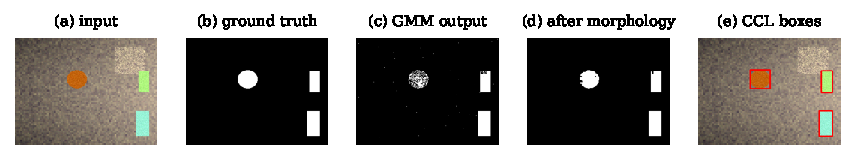
\includegraphics[width=0.86\textwidth]{fig_synthetic_qual.pdf}
\caption{Processing stages for frame 180 of the synthetic sequence (default
hardware model). The bimodal region in the upper right is already part of the
background.}
\label{fig:synq}
\end{figure*}
\begin{figure*}[!t]
\centering
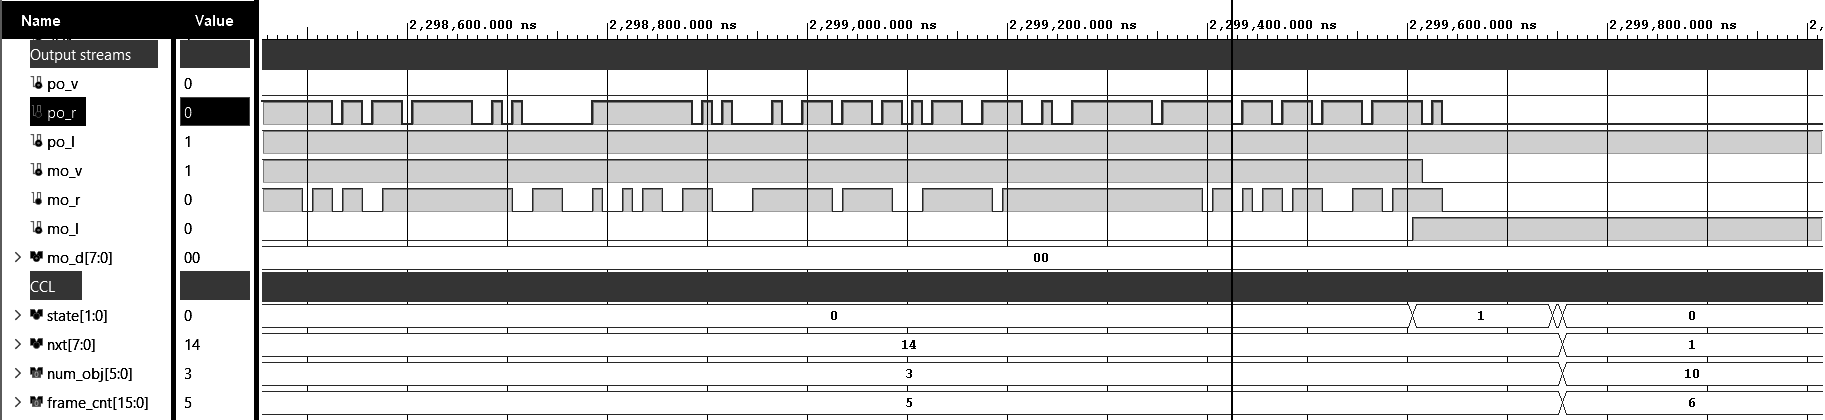
\includegraphics[width=0.85\textwidth]{fig_xsim.png}
\caption{Vivado behavioral simulation at the end of frame 5 ($160\times120$,
random back-pressure on both output streams). \texttt{mo\_l} marks the last mask
pixel. The CCL scans its labels (\texttt{state}\,=\,1) and publishes the object
table (\texttt{num\_obj} 3$\to$10, \texttt{frame\_cnt} 5$\to$6). Labeling
restarts at \texttt{nxt}\,=\,1.}
\label{fig:xsim}
\end{figure*}
A Python model reproduces every integer operation of the RTL, for any word
length, including rounding, saturation, ranking, label allocation, merge order
and the order of the object table. On every frame without label overflow, its
CCL is also checked against a breadth-first-search labeler.

The testbench checks itself. It configures the core over AXI4-Lite, changes the
learning-rate register every frame and streams frames with random valid gaps
(30\%) and random back-pressure on both outputs. The returned model is fed back
as the next frame's input. The masks, the object tables and the final model are
compared with the golden files. It runs with Icarus Verilog and with the Vivado
simulator.

The regression covers both word-length sets, all four morphology modes, and fast
and slow learning rates. It also has a case with label overflow, a 64-label
configuration and full $640\times480$ frames. A stand-alone test sends 400
random binary images through the CCL: noise, blobs, combs, U-shapes that merge
late, and rings. All cases match bit for bit.

The system-level test also passes in the Vivado simulator (xsim) before
implementation. Fig.~\ref{fig:xsim} shows the end of one frame in xsim. We also
ran the unchanged PYNQ driver against the RTL on a PC, with every DMA transfer
executed in Icarus. After the last mask pixel (TLAST), the CCL checks its 13
provisional labels in 13 clock cycles and publishes 10 objects. The end-of-frame
cost is therefore below 0.05\% of the frame time and at most $L=128$ cycles.

%=============================================================================
\section{Results}
%=============================================================================
\subsection{Resources and Throughput}

\begin{table}[!t]
\caption{Post-route resource utilization (Vivado 2025.2, XC7Z020)}
\label{tab:res}
\centering
\setlength{\tabcolsep}{3.6pt}
\begin{tabular}{@{}lrrrrr@{}}
\toprule
Module & LUT & LUTRAM & FF & DSP & BRAM\\
\midrule
GMM core (126 b)             & 1277 &   0 & 1094 & 6 & 0\\
Morphology (4 stages)        &  251 & 128 &  208 & 0 & 0\\
Single-pass CCL              & 1334 & 440 & 1110 & 0 & 0.5\\
AXI-Lite registers, glue     &  439 &   0 &  327 & 0 & 0\\
\midrule
Detector core (\texttt{mod\_top}) & 3277 & 568 & 2743 & 6 & 0.5\\
\ \ \% of XC7Z020            & 6.2  & 3.3 & 2.6  & 2.7 & 0.4\\
AXI DMA $\times2$            & 3300 &  32 & 5250 & 0 & 7\\
SmartConnect $\times2$ (HP0/1) & 3981 & 1006 & 7314 & 0 & 0\\
Full system (incl.\ GP0 path) & 11050 & 1606 & 16020 & 6 & 7.5\\
\ \ \% of XC7Z020            & 20.8 & 9.2 & 15.1 & 2.7 & 5.4\\
\bottomrule
\end{tabular}

\vspace{1pt}
{\footnotesize LUT = logic LUTs; BRAM in 36-kb tiles (RAMB18 = 0.5).}
\end{table}

Table~\ref{tab:res} lists the post-route resources. The complete detector core
uses 3.8k LUTs including LUTRAM. That is 7.2\% of the XC7Z020. The DMAs and the
SmartConnects take 2.2 times the logic of the detector. Each SmartConnect joins
the read and write master of one DMA on one HP port.

The GMM core needs 1281 LUTs and 6 DSP slices. A build without SmartConnects
needs 923 LUTs, and the difference is post-route register replication. The CCL
is the largest block, because its merger table updates all entries in parallel.
The design meets timing at 100\,MHz with a worst negative slack of
$+0.193$\,ns. The worst path is in the CCL. It runs from the row counter to the
enable of the merger table and takes 9.4\,ns over eight logic levels.

Without stalls, a $640\times480$ frame takes 309\,778 cycles. The pixels use
most of them. Another 2\,578 cycles cover pipeline fill, morphology flushing and
the CCL scan. That gives 3.10\,ms per frame, or 323\,frames/s at 100\,MHz.

When the 64-bit HP port runs at the same clock, the 16-byte model read limits
the system to about 50\,Mpixel/s, which is 160\,frames/s at VGA.

\begin{figure}[!t]
\centering
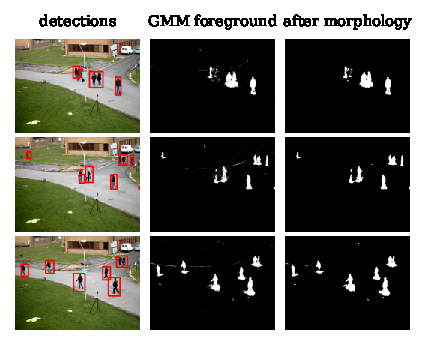
\includegraphics[width=\columnwidth]{fig_real_qual.pdf}
\caption{Real pedestrian sequence (OpenCV \texttt{vtest.avi}) resized to
$640\times480$, frames 60, 150 and 250. The boxes come from the bit-exact model
of the CCL unit.}
\label{fig:real}
\end{figure}

\subsection{Timing Closure}
\begin{table}[!t]
\caption{Timing closure at 100\,MHz (Vivado, post-route)}
\label{tab:timing}
\centering
\begin{tabular}{@{}lcc@{}}
\toprule
 & One-cycle CCL & Two-stage CCL\\
\midrule
Worst negative slack      & $-4.973$\,ns & $+0.193$\,ns\\
Failing endpoints         & 5713 & 0\\
Critical path             & CCL (14.5\,ns) & CCL (9.4\,ns)\\
Achievable clock          & $\approx$67\,MHz & 100\,MHz\\
CCL LUTs (incl.\ LUTRAM)  & 2683 & 1774\\
Detector core LUTs / DSPs & 4323 / 9 & 3849 / 6\\
\bottomrule
\end{tabular}
\end{table}

Table~\ref{tab:timing} shows the first implementation. All 5713 failing endpoints
were in the CCL. The critical path started at a neighbor register and went
through the 128-entry merger-table multiplexer, the label decision, the
feature-RAM address (fan-out 129), the feature read and two comparison chains,
ending at the feature write.

The two-stage CCL of Section~IV-C fixes this: it removes the table look-up and
the feature read from the labeling path, and it shrinks the CCL from 2683 to 1774
LUTs, because the parallel feature reads now use registered addresses. In the
GMM, the learning-rate look-up became constant comparisons, which saves 3 DSPs,
and the variance update was spread over three stages. The behavior is unchanged,
since the same bit-exact regression passes before and after.

\begin{table}[!t]
\caption{Comparison with the FPGA implementation of~\cite{genovese2014}}
\label{tab:cmp}
\centering
\setlength{\tabcolsep}{3pt}
\begin{tabular}{@{}lcccc@{}}
\toprule
 & \cite{genovese2014} & \multicolumn{2}{c}{This work, GMM} & This work\\
\cmidrule(lr){3-4}
 &  & Table I & default & full core\\
\midrule
Device           & Virtex-6 & Zynq-7020 & Zynq-7020 & Zynq-7020\\
Model bits/pixel & 99 & 99 & 126 & 126\\
Pipeline stages  & 1 & 5 & 5 & 5+\\
LUT / FF         & 788 / 363 & 553 / 512 & 1281 / 1094 & 3849 / 2743\\
DSP / BRAM       & 3 / 0 & 6 / 0 & 6 / 0 & 6 / 0.5\\
Clock (MHz)      & 189.3 & 100 & 100 & 100\\
Slack @100\,MHz  & -- & $+0.41$\,ns & $+0.19$\,ns & $+0.19$\,ns\\
Frames/s         & 91 HD & 48 HD$^\dagger$ & 48 HD$^\dagger$ & 323 VGA$^\dagger$\\
Energy/pixel     & 0.72\,nJ & 0.33\,nJ$^\ddagger$ & 0.43\,nJ$^\ddagger$ & 0.43\,nJ$^\ddagger$\\
\bottomrule
\end{tabular}

\vspace{1pt}
{\footnotesize $^\dagger$compute bound, 1 pixel/clock.
$^\ddagger$Vivado estimate, whole detector core.}
\end{table}

Table~\ref{tab:cmp} compares this work with the Virtex-6 design
of~\cite{genovese2014}. We built our GMM core with the same word lengths as
Table~I. It needs 553 LUTs, which is 30\% fewer than the 788 LUTs of the
reference. It needs more flip-flops (512), because of its five pipeline stages
and its stream control. It also uses three more DSP slices, because
$\lambda^2\sigma^2$ is a true multiplication here. The default 126-bit core needs
1281 LUTs.

Both versions meet 100\,MHz on the Artix-class fabric of the Zynq-7020, against
189\,MHz on Virtex-6 for~\cite{genovese2014}. The full core adds morphology and
blob analysis. Its estimated energy is 0.33 to 0.43\,nJ per pixel. The 0.72\,nJ
of~\cite{genovese2014} is of the same order, although the technologies and the
estimation methods differ.

\subsection{Accuracy}
The paper's metric, called ``MSE'', is the fraction of pixels classified
differently from the double-precision algorithm. Its target in~\cite{genovese2014}
is below 0.05. We report it together with the detection quality against exact
ground truth.

The test sequence is synthetic, with $320\times240$ pixels and 400 frames. It
contains a textured background, Gaussian noise ($\sigma=4$) and a slow global
illumination drift. A bimodal region switches randomly between two colors, and
three textured objects move. Metrics are collected after 60 frames. An object
counts as detected when a reported box overlaps its ground-truth box with
IoU $\ge 0.5$. All GMMs use $\alpha_w=2^{-7}$, $\lambda=2.5$, $T=0.7$ and $K=3$.
Closing and opening follow.

\begin{table}[!t]
\caption{Synthetic sequence: mismatch vs.\ float OpenCV GMM and detection quality}
\label{tab:acc}
\centering
\setlength{\tabcolsep}{2.6pt}
\begin{tabular}{@{}lccccc@{}}
\toprule
Method & MSE & Prec. & Rec. & F1 & Obj.\ rec.\\
\midrule
HW model, default (126 b)          & 0.0025 & 0.997 & 0.973 & 0.984 & 0.977\\
HW model, Table I of \cite{genovese2014} (99 b) & 0.0329 & 0.607 & 0.978 & 0.749 & 0.929\\
HW model, constant $\alpha_w$       & 0.0145 & 0.999 & 0.661 & 0.795 & 0.626\\
Float OpenCV GMM \cite{genovese2014} & 0      & 0.997 & 0.974 & 0.985 & 0.981\\
OpenCV MOG2 \cite{zivkovic2004}      & 0.0056 & 0.998 & 0.969 & 0.983 & 0.981\\
Float Stauffer--Grimson \cite{stauffer1999} & 0.0125 & 0.858 & 0.942 & 0.898 & 0.954\\
\bottomrule
\end{tabular}
\end{table}

Table~\ref{tab:acc} summarizes the comparison. With the default word lengths, the
hardware differs from the floating-point OpenCV GMM in only 0.25\% of the
pixels, and its detection quality is the same (F1 0.984 vs.\ 0.985).

The Table~I representation of~\cite{genovese2014} also stays below the 0.05
mismatch target, at 0.033. Its 8-bit weights have a problem, though. At
$\alpha_w=2^{-7}$ they cannot decay below a quarter of full scale. The coarser
variance adds more mismatches. After blob analysis the result is 14.8 false
boxes per frame and an F1 of 0.749. So a pixel-level mismatch target is not
enough when the mask feeds an object detector.

The warm-up schedule matters too. Without it, the background variances stay wide
for many frames, and recall drops to 0.66.

\begin{figure}[!t]
\centering
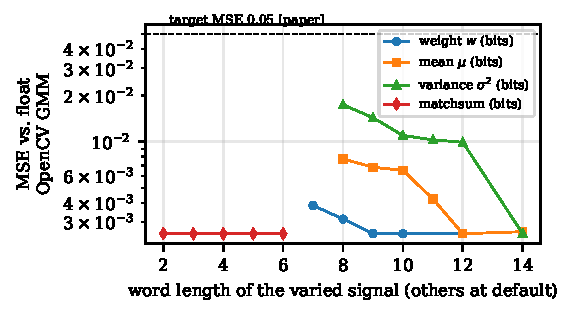
\includegraphics[width=\columnwidth]{fig_wordlength.pdf}
\caption{Word-length sensitivity (one signal varied, the others at the
default). The variance word length matters most, in agreement
with~\cite{genovese2014}.}
\label{fig:wl}
\end{figure}

Fig.~\ref{fig:wl} repeats the word-length study of~\cite{genovese2014} (Fig.~3
there), changing one signal at a time. We agree with that paper: the variance
has the strongest influence, and the matchsum is uncritical because it only sets
the weight of a new Gaussian.

Fig.~\ref{fig:synq} shows the processing stages for one frame. A single Gaussian
cannot represent the bimodal region, but the second mode of the mixture has
already absorbed it into the background.

\begin{table}[!t]
\caption{Post-processing (default hardware model)}
\label{tab:morph}
\centering
\setlength{\tabcolsep}{4pt}
\begin{tabular}{@{}lccccc@{}}
\toprule
Filter & Prec. & Recall & F1 & Obj.\ rec. & False boxes/fr.\\
\midrule
none              & 0.896 & 0.862 & 0.879 & 0.988 & 0.39\\
opening           & 1.000 & 0.746 & 0.855 & 0.726 & 1.36\\
closing           & 0.893 & 0.975 & 0.932 & 0.966 & 0.06\\
closing + opening & 0.997 & 0.973 & 0.984 & 0.977 & 0.04\\
\bottomrule
\end{tabular}
\end{table}

Table~\ref{tab:morph} shows why the filter is configurable. Opening alone breaks
textured objects into fragments. Closing followed by opening fills the holes and
removes the speckle, which gives 0.04 false boxes per frame.

A learning-rate sweep exposes a limit of power-of-two fixed-point updates. From
$\alpha_w=2^{-5}$ to $2^{-7}$ the hardware F1 is 0.935, 0.975 and 0.984, close to
the float model (0.939, 0.985, 0.985). For $2^{-8}$ and $2^{-9}$ it falls to
0.600 and 0.427, while the float model keeps 0.966 and 0.937. The background
Gaussians then have $\alpha_k\approx\alpha_w$. Updates smaller than half an LSB of
the mean and variance are lost, and the background stops following the
illumination drift.

On the real sequence (Fig.~\ref{fig:real}, 300 frames) the hardware model differs
from the floating-point GMM in 0.26\% of the pixels with the default word
lengths, and in 1.9\% with the Table~I lengths. It reports 7.4 objects per frame
on average and 18 at most. In 4 of the 300 frames, more than 127 provisional
labels were needed and the overflow flag was raised. Setting
\texttt{LBL\_W}\,=\,8 removes this, at the cost of a larger CCL.

\begin{table}[!t]
\caption{Implementation and on-board results (PYNQ-Z2, $640\times480$)}
\label{tab:board}
\centering
\begin{tabular}{@{}lr@{}}
\toprule
Metric & Value\\
\midrule
PL clock / worst negative slack (Vivado)     & 100\,MHz / $+0.193$\,ns\\
Power, core / DMAs / SmartConn.\ (est.)      & 43 / 19 / 53\,mW\\
Total on-chip power, of which PS (est.)      & 1.524\,W / 1.264\,W\\
PL + DMA time per frame (measured, 300 fr.)  & 8.71\,ms\\
Frame rate, hardware path                    & 114.8\,fps\\
Frame rate, end-to-end with Python control   & 34.9\,fps\\
ARM-only software (MOG2 + morphology + CCL)  & 7.4\,fps\\
Speed-up over ARM software, HW / end-to-end  & 15.5$\times$ / 4.7$\times$\\
Bit-exact check vs.\ model (\texttt{--verify}) & pass (20 frames)\\
\bottomrule
\end{tabular}
\end{table}

\subsection{On-Board Measurements}
On the board, the mask, the model and the object table match the reference
model bit for bit on the first 20 frames of the pedestrian sequence. The hardware
path needs 8.71\,ms per VGA frame, which is 15.5 times less than OpenCV MOG2 with
the same post-processing on the ARM (135.4\,ms). The datapath alone needs
3.10\,ms, and memory takes the rest. Each frame moves 4.9\,MB of model in each
direction through HP0, which is 70\% of the port's peak bandwidth. End to end,
Python video decoding limits the system to 34.9\,fps. The Vivado power estimate
is vectorless. It gives 1.26\,W to the processing system and the DDR interface,
and only 43\,mW to the detector core.

\subsection{Discussion and Limitations}
Memory sets the throughput: the model stream (32\,B per pixel) on one 64-bit HP
port bounds the system to about 50\,Mpixel/s, half the datapath rate.
Compressing the model or splitting it over two HP ports would raise this limit.

The row buffers support frames up to 1024 pixels wide, so HD video needs
\texttt{MAX\_W}\,=\,2048 and possibly $L=256$ labels. Learning rates below
$2^{-7}$ would need more bits for the mean and variance, or stochastic rounding.

%=============================================================================
\section{Conclusion}
%=============================================================================
We built a complete moving object detector on a Zynq SoC, based on the
OpenCV GMM formulation of Genovese and Napoli. We extended their background
identification circuit with configurable morphological filtering, single-pass
connected component labeling and DMA-based system integration.

A bit-exact verification flow and a word-length study gave two results. First,
the published 99-bit representation meets its pixel-level mismatch target, but it
degrades object-level detection. Second, a 126-bit representation that fits one
DMA word matches the floating-point algorithm within 0.25\% of the pixels. With
a software warm-up schedule for the learning rate, it reaches an F1 score of
0.984. The core uses 7.2\% of the XC7Z020 LUTs and runs at 100\,MHz after we
split the CCL into a labeling stage and a feature stage. On the PYNQ-Z2 it
processes VGA video at 115\,frames/s, 15.5 times faster than the ARM software.
Future work includes
compressing the model stream, adding shadow detection and tracking objects on the
ARM cores.

\begin{thebibliography}{99}
\bibitem{stauffer1999}
C.~Stauffer and W.~E.~L. Grimson, ``Adaptive background mixture models for
real-time tracking,'' in \emph{Proc. IEEE Conf. Computer Vision and Pattern
Recognition (CVPR)}, vol.~2, 1999, pp.~246--252.

\bibitem{kaew2001}
P.~KaewTraKulPong and R.~Bowden, ``An improved adaptive background mixture
model for real-time tracking with shadow detection,'' in \emph{Proc. Eur.
Workshop Advanced Video Based Surveillance Systems}, 2001, pp.~1--5.

\bibitem{genovese2014}
M.~Genovese and E.~Napoli, ``ASIC and FPGA implementation of the Gaussian
mixture model algorithm for real-time segmentation of high definition
video,'' \emph{IEEE Trans. VLSI Syst.}, vol.~22, no.~3, pp.~537--547, 2014.

\bibitem{rosenfeld1966}
A.~Rosenfeld and J.~L. Pfaltz, ``Sequential operations in digital picture
processing,'' \emph{J. ACM}, vol.~13, no.~4, pp.~471--494, 1966.

\bibitem{ug585}
Xilinx, ``Zynq-7000 SoC technical reference manual,'' UG585.

\bibitem{zivkovic2004}
Z.~Zivkovic, ``Improved adaptive Gaussian mixture model for background
subtraction,'' in \emph{Proc. 17th Int. Conf. Pattern Recognition (ICPR)},
vol.~2, 2004, pp.~28--31.

\bibitem{jiang2009}
H.~Jiang, H.~Ard\"o, and V.~\"Owall, ``A hardware architecture for real-time
video segmentation utilizing memory reduction techniques,'' \emph{IEEE Trans.
Circuits Syst. Video Technol.}, vol.~19, no.~2, pp.~226--236, 2009.

\bibitem{kristensen2008}
F.~Kristensen, H.~Hedberg, H.~Jiang, P.~Nilsson, and V.~\"Owall, ``An
embedded real-time surveillance system: Implementation and evaluation,''
\emph{J. Signal Process. Syst.}, vol.~52, no.~1, pp.~75--94, 2008.

\bibitem{genovese2012}
M.~Genovese and E.~Napoli, ``FPGA-based architecture for real time
segmentation and denoising of HD video,'' \emph{J. Real-Time Image
Process.}, 2012.

\bibitem{kryjak2011}
T.~Kryjak, M.~Komorkiewicz, and M.~Gorgon, ``Real-time moving object detection
for video surveillance system in FPGA,'' in \emph{Proc. Conf. Design and
Architectures for Signal and Image Processing (DASIP)}, 2011.

\bibitem{bailey2007}
D.~G. Bailey and C.~T. Johnston, ``Single pass connected components
analysis,'' in \emph{Proc. Image and Vision Computing New Zealand}, 2007,
pp.~282--287.

\bibitem{johnston2008}
C.~T. Johnston and D.~G. Bailey, ``FPGA implementation of a single pass
connected components algorithm,'' in \emph{Proc. 4th IEEE Int. Symp.
Electronic Design, Test and Applications (DELTA)}, 2008, pp.~228--231.

\bibitem{ma2008}
N.~Ma, D.~G. Bailey, and C.~T. Johnston, ``Optimised single pass connected
components analysis,'' in \emph{Proc. Int. Conf. Field-Programmable
Technology (FPT)}, 2008.

\bibitem{bailey2019}
D.~G. Bailey and M.~J. Klaiber, ``Zig-zag based single-pass connected
components analysis,'' \emph{J. Imaging}, vol.~5, no.~4, art.~45, 2019.
\end{thebibliography}

\end{document}
